%!TEX root = ../template.tex
%%%%%%%%%%%%%%%%%%%%%%%%%%%%%%%%%%%%%%%%%%%%%%%%%%%%%%%%%%%%%%%%%%%%
%% benchmark.tex
%% NOVA thesis document file
%%
%% Chapter with a short latex tutorial and examples
%%%%%%%%%%%%%%%%%%%%%%%%%%%%%%%%%%%%%%%%%%%%%%%%%%%%%%%%%%%%%%%%%%%%

\typeout{NT FILE benchmark.tex}

\chapter{Benchmark}
\label{cha:benchmark}

In this chapter, we cover the third (collaborative) contribution from this dissertation, which consists in the backend and corresponding client for an edge-enabled application, intended to be used as a benchmark for service deployment systems, which may in turn, rely on the devised framework. This benchmark, which we called PouchBeasts, is composed by multiple independent microservices, and aims to provide similar functionality to PokemonGO \todo{cite pokemonGO} (although with fewer features), but in a distributed manner.

In this system, users registered in the system own a set of beasts, which they can expand by catching or acquiring new ones. Beasts are collectible items with different properties (such as attack, health, among others) that appear in random geographical locations, where they may be caught by the users (if the users' geographical location is within a certain bound of the beast to be caught). Then, users can perform two main actions with their owned beasts, the first is to battle with other users (and their beasts) and the second action is to join other users in a cooperative battle against a computer-controled beast. During these battles, users must signal their beasts to either attack or defend and can use items on their beasts, which can have multiple effects, such as reviving a dead beast, healing a certain amount of health, among other uses. These items may be traded with other users, or acquired from a shop using tokens, which in turn are acquired through coins bought via microtransactions.

\begin{figure}[htbp]
    \centering
    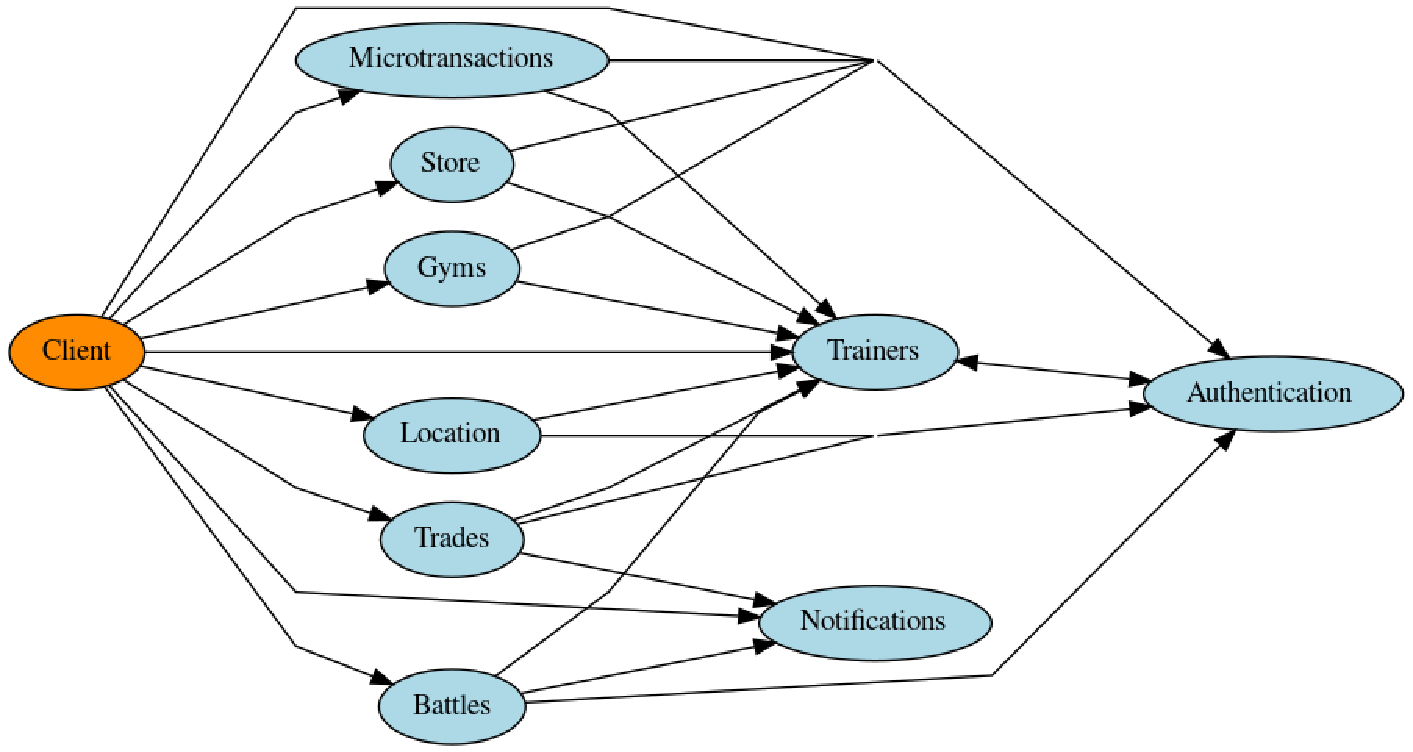
\includegraphics[width=\textwidth]{Chapters/benchmark/figures/interaction-diagram.pdf}
    \caption{An overview of the architecture of PouchBeasts}
    \label{fig:pouchbeasts-overview}
\end{figure}

Provided with a brief overview of the system functionality, we now explain each of the microservices that work together to satisfy the aforementioned requirements. This benchmark, as illustrated in the interaction diagram of figure \ref{fig:pouchbeasts-overview}, is composed by nine microservices and a client to access them. We now provide a brief overview of each microservice and its role within the system:

\begin{enumerate}
    \item The first and most used microservice of the system is called \textbf{Trainers}, this microservice essentially stores all the data related to the users and their owned beasts. In addition, it verifies the tokens issued by the authentication microservice in regard to the recency of the information carried in the token. This service makes use of a mongoDB database to store these records in permanent storage and maintain data consistency across microservices.
    
    \item The next microservice is called \textbf{Authentication}, which only has the purpose of generating new authentication tokens for the users to use when interacting with other services. These tokens contain a hash of the owned beasts, so that other servers can verify their authenticity and recency without having to fetch the users' pokemons on each interaction.

    \item Following, we have the \textbf{Gyms} and \textbf{Battles} services, these allow players to perform combats with their obtained beasts. In the case of the gyms service, it manages entities in the system denominated gymnasiums, which have an assigned geographical locations. In this service, if a user is within a geographical distance of the gymnasium, it may perform battles alongside other trainers against a single beast controlled by the computer. The \textbf{Battles} service is a service that allows users to use their beasts to combat other users, battles in this service can start either via a queueing system, where players wait for another random user to start the battle, or alternatively via challenging other known users (via a notification).
    
    \item Then, we have the \textbf{Store} and \textbf{Microtransactions} services, the objective behind these is simple, the Microtransactions service provides a way for users to obtain currency via small value transactions, which then can the be used in the store service for buying new items to use in the beasts (e.g. for healing or reviving a beast which has little or no health).

    \item Users may also change their items via the \textbf{Trades} service, this service grants users the possibility to exchange their items with other users in the system. In order to use this system, a user must invite another currently active user via a notification (which can optionally be accepted by the target user).

    \item The service responsible for handling all of the previously mentioned notifications is called \textbf{Notifications}. This service is essentially tasked with receiving notifications from connected users and propagating them towards the target user. As there may be multiple notification services executing concurrently and users may connect to any of the available servers, a notification may be emitted for a user not connected to the same server. To prevent these notifications from being lost, this service makes use of a Kafka backend, which it uses to propagate messages for nodes that are connected to different notification servers.

    \item The last implemented microservice is called \textbf{Location} service, this service is responsible for managing the geographical locations of the users using the system, the generation and management of the generated beasts (for users to catch), and the locations of gymnasiums in a certain geographical area. In order to prevent multiple location services from managing overlapping geographical areas, and to facilitate the insertion and decommission of new location servers, we assign portions of the geographical area to certain servers using S2 cells \todo{cite}. S2 cells provide a framework for decomposing the a sphere (in our case, the earth) into a hierarchy of cells, where each S2 cell is quadrilateral bounded by four geodesics. The top level of the hierarchy is obtained by projecting the six faces of a cube onto the earth, and lower levels are obtained by subdividing each cell into four children recursively. An example of two of the six face cells (one of which has been subdivided multiple times) can be observed in figure \ref{fig:pouchbeasts-s2cells}, obtained from \todo{cite}. This service makes use of S2 cells to (1) assign portions of the earth to servers in a way that does not create geographical discontinuities, (2) to index efficiently the locations of trainers, gyms and generated beasts, which allows the service to, based on cell centred on a user-provided location, determine the beasts and gyms to return to the user, (3) in the case a user's location is in the boundary of two (or more) location servers, S2 cells are also used to decide to which server(s) the user should connect to, so that it does not receive only a portion of the results for its correspondent geographical area, and finally (4) to allow a dynamic subdivision and collapse of geographical regions to instantiate or decommission location servers.

\end{enumerate}

\begin{figure}[htbp]
    \centering
    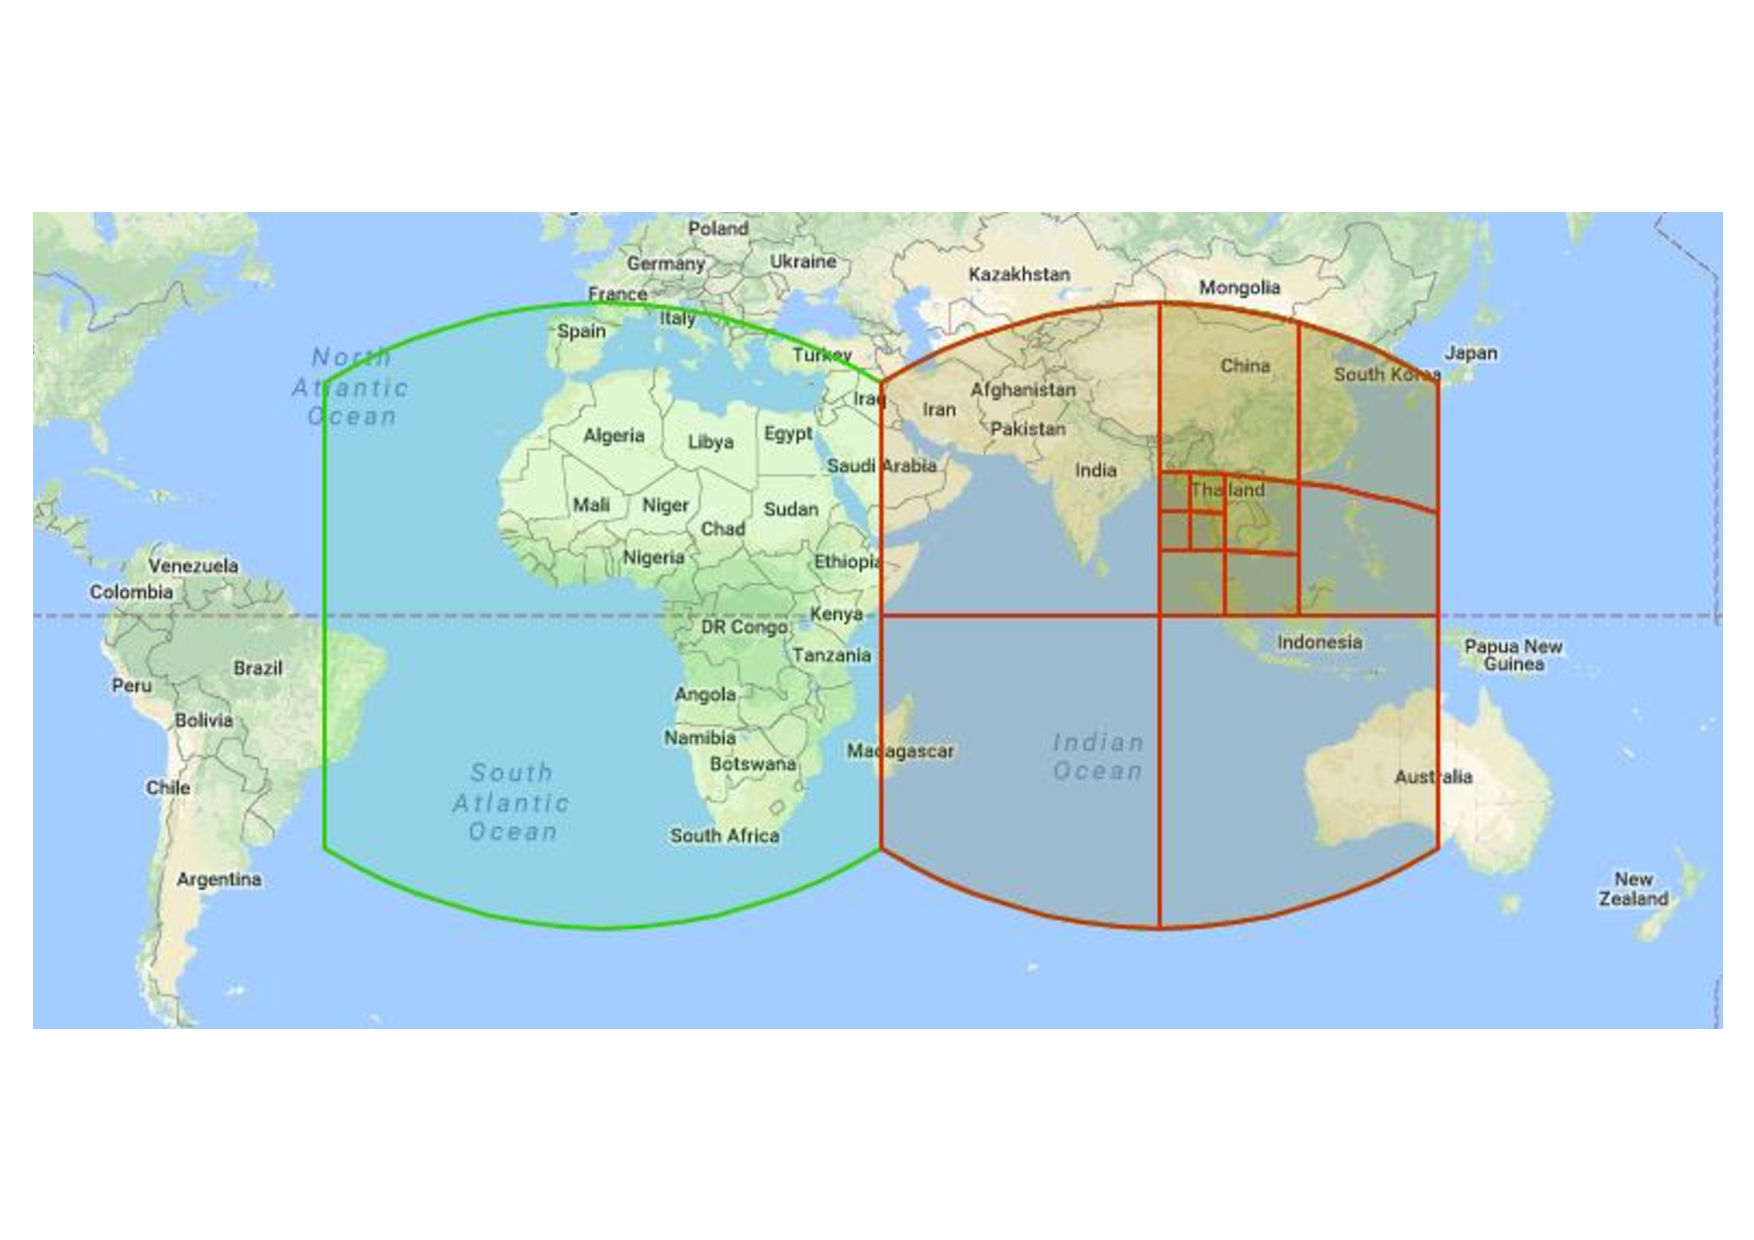
\includegraphics[width=\textwidth]{Chapters/benchmark/figures/s2_cells.pdf}
    \caption{Example of S2 cell hierarchy}
    \label{fig:pouchbeasts-s2cells}
\end{figure}